% Festlegung des Allgemeinen Dokumentenformats
\documentclass[a4paper,12pt,headsepline,parskip=half]{scrartcl}

% Umlaute unter UTF8 nutzen
\usepackage[utf8]{inputenc}

% Variablen
%Variablen welche innerhalb der gesamten Arbeit zur Verfügung stehen sollen
\newcommand{\titleDocument}{Projekt Programmierung}
\newcommand{\subjectDocument}{im Studiengang <Studiengang>}
\newcommand{\Matrikelnummer}{50855}
\newcommand{\Thema}{Entwicklung eines Anwesenheitsplaners für das SMK}
\newcommand{\Abgabedatum}{19.07.2023}
\newcommand{\Studiengang}{Informatik}


% weitere Pakete
% Grafiken aus PNG Dateien einbinden
\usepackage{graphicx}

% Deutsche Sonderzeichen und Silbentrennung nutzen
\usepackage[ngerman]{babel}

% Eurozeichen einbinden
\usepackage[right]{eurosym}

% Zeichenencoding
\usepackage[T1]{fontenc}

\usepackage{lmodern}

% floatende Bilder ermöglichen
%\usepackage{floatflt}

% mehrseitige Tabellen ermöglichen
\usepackage{longtable}

% Unterstützung für Schriftarten
%\newcommand{\changefont}[3]{ 
%\fontfamily{#1} \fontseries{#2} \fontshape{#3} \selectfont}

% Packet für Seitenrandabständex und Einstellung für Seitenränder
\usepackage{geometry}
\geometry{left=3.5cm, right=2cm, top=2.5cm, bottom=2cm}

% Paket für Boxen im Text
\usepackage{fancybox}

% bricht lange URLs "schön" um
\usepackage[hyphens,obeyspaces,spaces]{url}

% Paket für Textfarben
\usepackage{color}

% Mathematische Symbole importieren
\usepackage{amssymb}

% auf jeder Seite eine Überschrift (alt, zentriert)
%\pagestyle{headings}

% erzeugt Inhaltsverzeichnis mit Querverweisen zu den Abschnitten (PDF Version)
\usepackage[bookmarksnumbered,pdftitle={\titleDocument},hyperfootnotes=false]{hyperref}
%\hypersetup{colorlinks, citecolor=red, linkcolor=blue, urlcolor=black}
%\hypersetup{colorlinks, citecolor=black, linkcolor= black, urlcolor=black}

% neue Kopfzeilen mit fancypaket
\usepackage{fancyhdr} %Paket laden
\pagestyle{fancy} %eigener Seitenstil
\fancyhf{} %alle Kopf- und Fußzeilenfelder bereinigen
\fancyhead[L]{\nouppercase{\leftmark}} %Kopfzeile links
\fancyhead[C]{} %zentrierte Kopfzeile
\fancyhead[R]{\thepage} %Kopfzeile rechts
\renewcommand{\headrulewidth}{0.4pt} %obere Trennlinie
%\fancyfoot[C]{\thepage} %Seitennummer
%\renewcommand{\footrulewidth}{0.4pt} %untere Trennlinie

% für Tabellen
\usepackage{array}

% Runde Klammern für Zitate
%\usepackage[numbers,round]{natbib}

% Festlegung Art der Zitierung - Havardmethode: Abkuerzung Autor + Jahr
\bibliographystyle{alphadin}

% Schaltet den zusätzlichen Zwischenraum ab, den LaTeX normalerweise nach einem Satzzeichen einfügt.
%\frenchspacing

% Paket für Zeilenabstand
\usepackage{setspace}

% für Bildbezeichner
\usepackage{capt-of}

% für Stichwortverzeichnis
\usepackage{makeidx}

%Konfiguriere das Inhaltsverzeichnis
\usepackage{tocbasic}
\DeclareTOCStyleEntries[
  raggedentrytext,
  numwidth=0pt,
  numsep=1ex,
  dynnumwidth,
]{tocline}{chapter,section,subsection,subsubsection,paragraph,subparagraph}
\DeclareTOCStyleEntries[
  indent=0pt,
  linefill=\TOCLineLeaderFill,
]{tocline}{section,subsection,subsubsection,paragraph,subparagraph}
\DeclareTOCStyleEntries[
  indent=10pt,
]{tocline}{subsection,subsubsection,paragraph,subparagraph}

% für Listings
\usepackage{listings}
\lstset{numbers=left, numberstyle=\tiny, numbersep=5pt, keywordstyle=\color{black}\bfseries, stringstyle=\ttfamily,showstringspaces=false,basicstyle=\footnotesize,captionpos=b}
\lstset{language=java}

% Indexerstellung
\makeindex

% Abkürzungsverzeichnis
\usepackage[german]{nomencl}
\let\abbrev\nomenclature

% Abkürzungsverzeichnis LiveTex Version
% Titel des Abkürzungsverzeichnisses
\renewcommand{\nomname}{Abkürzungsverzeichnis}
% Abstand zwischen Abkürzung und Erläuterung
\setlength{\nomlabelwidth}{.25\textwidth}
% Zwischenraum zwischen Abkürzung und Erläuterung mit Punkten
\renewcommand{\nomlabel}[1]{#1 \dotfill}
% Variation des Abstandes der einzelnen Abkürzungen zu einander
\setlength{\nomitemsep}{-\parsep}
% Index mit Abkürzungen erzeugen
\makenomenclature
%\makeglossary

% Abkürzungsverzeichnis TeTEX Version
% \usepackage[german]{nomencl}
% \makenomenclature
% %\makeglossary
% \renewcommand{\nomname}{Abkürzungsverzeichnis}
% \AtBeginDocument{\setlength{\nomlabelwidth}{.25\columnwidth}}
% \renewcommand{\nomlabel}[1]{#1 \dotfill}
% \setlength{\nomitemsep}{-\parsep}

% Optional: Einzelne Zeilen am Anfang einer Seite unterdrücken (Schusterjungen)
% \clubpenalty = 10000
% Optional: Einzelne Zeilen am Ende einer Seite unterdrücken (Hurenkinder)
% \widowpenalty = 10000
% \displaywidowpenalty = 10000

\begin{document}
% hier werden die Trennvorschläge inkludiert
%hier müssen alle Wörter rein, welche Latex von sich auch nicht korrekt trennt bzw. bei denen man die genaue Trennung vorgeben möchte
\hyphenation{
Film-pro-du-zen-ten
Lux-em-burg
Soft-ware-bau-steins
zeit-in-ten-siv
}


% Schriftart Helvetica verwenden
%\usepackage{helvet}
%\renewcommand\familydefault{\sfdefault}

% Leere Seite am Anfang
\thispagestyle{empty} % erzeugt Seite ohne Kopf- / Fusszeile
\mbox{}
\newpage

% Titelseite %
\thispagestyle{empty}


\begin{figure}[t]
 \centering
 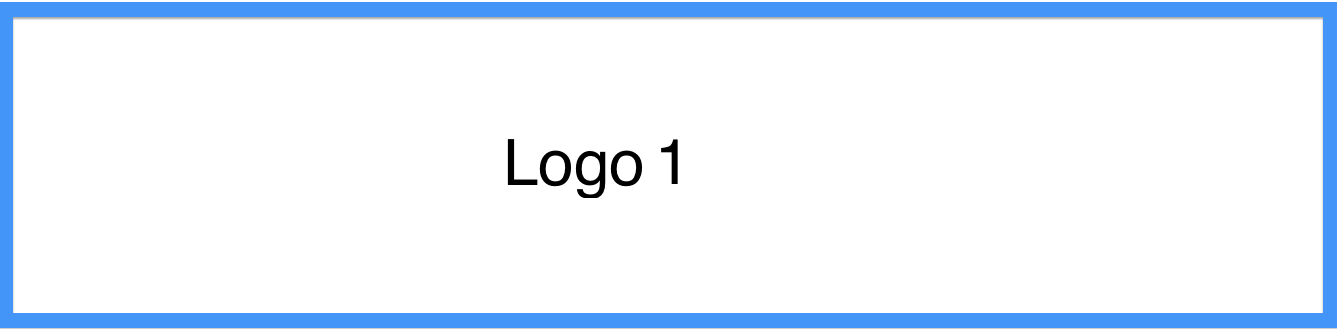
\includegraphics[width=0.6\textwidth]{abb/logo1}
~~~~~~~~~~
 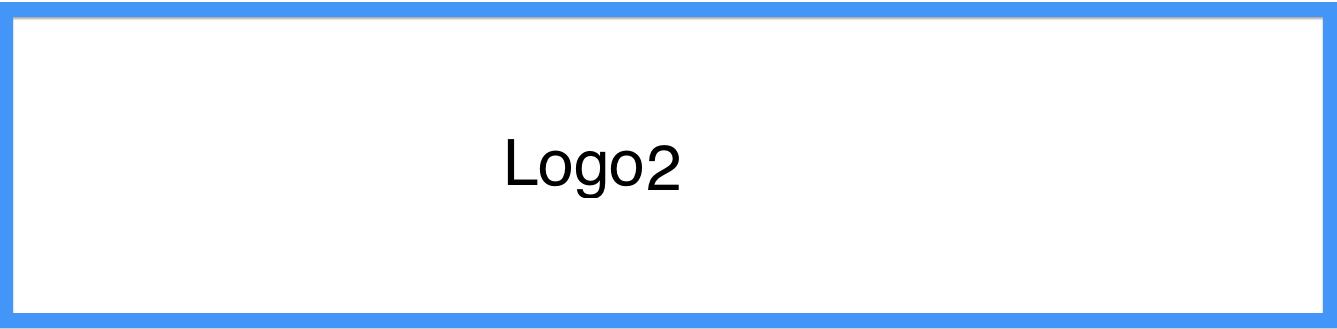
\includegraphics[width=0.3\textwidth]{abb/logo2}
\end{figure}


\begin{verbatim}


\end{verbatim}

\begin{center}
\Large{Fachhochschule <Name>}\\
\Large{- Campus <Name> -}\\
\end{center}


\begin{center}
\Large{Fakultät für <Fachrichtung>}
\end{center}
\begin{verbatim}




\end{verbatim}
\begin{center}
\doublespacing
\textbf{\LARGE{\titleDocument}}\\
\singlespacing
\begin{verbatim}

\end{verbatim}
\textbf{{~\subjectDocument~-~Schwerpunkt <Schwerpunktfach>}}
\end{center}
\begin{verbatim}

\end{verbatim}
\begin{center}

\end{center}
\begin{verbatim}

\end{verbatim}
\begin{center}
\textbf{zur Erlangung des akademischen Grades \\ Bachelor / Master of Science}
\end{center}
\begin{verbatim}






\end{verbatim}
\begin{flushleft}
\begin{tabular}{llll}
\textbf{Thema:} & & <Thema der Arbeit> & \\
& & \\
\textbf{Autor:} & & Name <name@mail.de>& \\
& & MatNr. 12345... & \\
& & \\
\textbf{Version vom:} & & \today &\\
& & \\
\textbf{1. Betreuerin:} & & Prof. Dr. X &\\
\textbf{2. Betreuer:} & & Prof. Dr. Y &\\
\end{tabular}
\end{flushleft}


% römische Numerierung
\pagenumbering{roman}

% 1.5 facher Zeilenabstand
\onehalfspacing

\newpage

% Sperrvermerk
\thispagestyle{empty}
\section*{Sperrvermerk}
\textcolor{red}{
Die vorliegende Arbeit beinhaltet interne und vertrauliche Informationen der Firma <Firmenname>.
Die Weitergabe des Inhalts der Arbeit im Gesamten oder in Teilen sowie das Anfertigen
von Kopien oder Abschriften - auch in digitaler Form - sind grundsätzlich untersagt.
Ausnahmen bedürfen der schriftlichen Genehmigung der Firma <Firmenname>.
}


\newpage

% Einleitung / Abstract
\thispagestyle{empty}
\section*{Zusammenfassung}

Hier steht der Text, welcher den Inhalte der Arbeit zusammenfasst...

Lorem ipsum dolor sit amet, consetetur sadipscing elitr, sed diam nonumy eirmod tempor invidunt ut labore et dolore magna aliquyam erat, sed diam voluptua. At vero eos et accusam et justo duo dolores et ea rebum. Stet clita kasd gubergren, no sea takimata sanctus est Lorem ipsum dolor sit amet. Lorem ipsum dolor sit amet, consetetur sadipscing elitr, sed diam nonumy eirmod tempor invidunt ut labore et dolore magna aliquyam erat, sed diam voluptua. At vero eos et accusam et justo duo dolores et ea rebum. Stet clita kasd gubergren, no sea takimata sanctus est Lorem ipsum dolor sit amet.

\section*{Abstract}

Here goes the English text which summarizes the content of the thesis...

Lorem ipsum dolor sit amet, consetetur sadipscing elitr, sed diam nonumy eirmod tempor invidunt ut labore et dolore magna aliquyam erat, sed diam voluptua. At vero eos et accusam et justo duo dolores et ea rebum. Stet clita kasd gubergren, no sea takimata sanctus est Lorem ipsum dolor sit amet. Lorem ipsum dolor sit amet, consetetur sadipscing elitr, sed diam nonumy eirmod tempor invidunt ut labore et dolore magna aliquyam erat, sed diam voluptua. At vero eos et accusam et justo duo dolores et ea rebum. Stet clita kasd gubergren, no sea takimata sanctus est Lorem ipsum dolor sit amet.


% einfacher Zeilenabstand
\singlespacing

\newpage
% Seitenzählung bei Inhaltsverzeichnis beginnen
\setcounter{page}{1}

% Inhaltsverzeichnis anzeigen
\thispagestyle{empty}
\tableofcontents

\newpage
% das Abbildungsverzeichnis
% Verion 1: Abbildungsverzeichnis MIT führender Nummberierung endgueltig anzeigen
\listoffigures
% Abbildungsverzeichnis soll im Inhaltsverzeichnis auftauchen
\addcontentsline{toc}{section}{Abbildungsverzeichnis}

% Verion 2: Abbildungsverzeichnis OHNE führende Nummberierung endgueltig anzeigen
%\begingroup
%\renewcommand\numberline[1]{}
%\listoffigures
%\endgroup


% das Tabellenverzeichnis
\newpage
% \fancyhead[L]{Abbildungsverzeichnis / Abkürzungsverzeichnis} %Kopfzeile links
% Tabellenverzeichnis endgültig anzeigen
\listoftables
% Tabellenverzeichnis soll im Inhaltsverzeichnis auftauchen
\addcontentsline{toc}{section}{Tabellenverzeichnis}

%% WORKAROUND für Listings
%\makeatletter% --> De-TeX-FAQ
%\renewcommand*{\lstlistoflistings}{%
%  \begingroup
%    \if@twocolumn
%      \@restonecoltrue\onecolumn
%    \else
%      \@restonecolfalse
%    \fi
%    \lol@heading
%    \setlength{\parskip}{\z@}%
%    \setlength{\parindent}{\z@}%
%    \setlength{\parfillskip}{\z@ \@plus 1fil}%
%    \@starttoc{lol}%
%    \if@restonecol\twocolumn\fi
%  \endgroup
%}
%\makeatother% --> \makeatletter
% das Listingverzeichnis
\newpage
\fancyhead[L]{Listingverzeichnis} %Kopfzeile links
\renewcommand{\lstlistlistingname}{Listingverzeichnis}
\lstlistoflistings
% Listingverzeichnis soll im Inhaltsverzeichnis auftauchen
\addcontentsline{toc}{section}{Listingverzeichnis}
%%%%

% das Abkürzungsverzeichnis
\newpage
% das Abkürzungsverzeichnis ausgeben
\fancyhead[L]{Abkürzungsverzeichnis} %Kopfzeile links
\nomenclature{UGC}{User Generated Content}
\nomenclature{CSS}{Cascading Style Sheets}
\nomenclature{JS}{JavaScript}
\nomenclature{SQL}{Structured Query Language}
\nomenclature{GPL}{GNU General Public License}
\nomenclature{GNU}{GNU is not Unix}
\nomenclature{LGPL}{GNU Lesser General Public License}
\nomenclature{XMPP}{Extensible Messaging and Presence Protocol}
\nomenclature{IM}{Instant Message}
\nomenclature{CMS}{Content Management System}
\nomenclature{RSS}{Really Simple Syndication}
\nomenclature{JSON}{JavaScript Object Notation}
\nomenclature{HTML}{Hypertext Markup Language}
\nomenclature{TDD}{Test-driven development}
\nomenclature{GUI}{Graphical User Interface}
\nomenclature{KPI}{Key Performance Indicator}
\nomenclature{WWW}{World Wide Web}
\nomenclature{OCR}{Optical Character Recognition}
\nomenclature{ERM}{Entity Relationship Modell}

\printnomenclature[3cm]
% Abkürzungsverzeichnis soll im Inhaltsverzeichnis auftauchen
\addcontentsline{toc}{section}{Abkürzungsverzeichnis}


%%%%%%% EINLEITUNG %%%%%%%%%%%%
\newpage
\fancyhead[L]{\nouppercase{\leftmark}} %Kopfzeile links

% 1,5 facher Zeilenabstand
\onehalfspacing

% arabische Seitennummerierung ab hier
\pagenumbering{arabic}

% Alternative Einbindung des Abstract in Kapitel "0" falls gewünscht
%\setcounter{section}{-1}
%\setcounter{page}{0}

% Option: Einbindung abstract
%\section*{Zusammenfassung}

Hier steht der Text, welcher den Inhalte der Arbeit zusammenfasst...

Lorem ipsum dolor sit amet, consetetur sadipscing elitr, sed diam nonumy eirmod tempor invidunt ut labore et dolore magna aliquyam erat, sed diam voluptua. At vero eos et accusam et justo duo dolores et ea rebum. Stet clita kasd gubergren, no sea takimata sanctus est Lorem ipsum dolor sit amet. Lorem ipsum dolor sit amet, consetetur sadipscing elitr, sed diam nonumy eirmod tempor invidunt ut labore et dolore magna aliquyam erat, sed diam voluptua. At vero eos et accusam et justo duo dolores et ea rebum. Stet clita kasd gubergren, no sea takimata sanctus est Lorem ipsum dolor sit amet.

\section*{Abstract}

Here goes the English text which summarizes the content of the thesis...

Lorem ipsum dolor sit amet, consetetur sadipscing elitr, sed diam nonumy eirmod tempor invidunt ut labore et dolore magna aliquyam erat, sed diam voluptua. At vero eos et accusam et justo duo dolores et ea rebum. Stet clita kasd gubergren, no sea takimata sanctus est Lorem ipsum dolor sit amet. Lorem ipsum dolor sit amet, consetetur sadipscing elitr, sed diam nonumy eirmod tempor invidunt ut labore et dolore magna aliquyam erat, sed diam voluptua. At vero eos et accusam et justo duo dolores et ea rebum. Stet clita kasd gubergren, no sea takimata sanctus est Lorem ipsum dolor sit amet.

%\newpage

% einzelne Kapitel werden hier eingebunden
\input{1_einleitung}
\newpage

\section{Hauptabschnitt}\label{hauptabschnitt}

Text des ersten Abschnitts... Lorem ipsum dolor sit amet, consetetur sadipscing elitr, sed diam nonumy eirmod tempor invidunt ut labore et dolore magna aliquyam erat, sed diam voluptua. At vero eos et accusam et justo duo dolores et ea rebum. Stet clita kasd gubergren, no sea takimata sanctus est Lorem ipsum dolor sit amet. Lorem ipsum dolor sit amet, consetetur sadipscing elitr, sed diam nonumy eirmod tempor invidunt ut labore et dolore magna aliquyam erat, sed diam voluptua. At vero eos et accusam et justo duo dolores et ea rebum. Stet clita kasd gubergren, no sea takimata sanctus est Lorem ipsum dolor sit amet.

\subsection{Unterabschnitt 1}\label{unterabschnitt_1}

Erstes Unterabschnitt

\subsection{Unterabschnitt 2}\label{unterabschnitt_2}

Zweites Unterabschnitt

\subsection{Unterabschnitt 3}\label{unterabschnitt_3}

Drittes Unterabschnitt

\newpage

\section{Weiterer Hauptabschnitt}\label{hauptabschnitt_2}

Text des zweiten Abschnitts... Lorem ipsum dolor sit amet, consetetur sadipscing elitr, sed diam nonumy eirmod tempor invidunt ut labore et dolore magna aliquyam erat, sed diam voluptua. At vero eos et accusam et justo duo dolores et ea rebum. Stet clita kasd gubergren, no sea takimata sanctus est Lorem ipsum dolor sit amet. Lorem ipsum dolor sit amet, consetetur sadipscing elitr, sed diam nonumy eirmod tempor invidunt ut labore et dolore magna aliquyam erat, sed diam voluptua. At vero eos et accusam et justo duo dolores et ea rebum. Stet clita kasd gubergren, no sea takimata sanctus est Lorem ipsum dolor sit amet.

\newpage

% hier können weitere Kapitel angelegt und eingetragen werden
% ....

\section{Ausblick}\label{ausblick}

Text des Ausblicks - sofern dies in der Arbeit gewünscht ist... Lorem ipsum dolor sit amet, consetetur sadipscing elitr, sed diam nonumy eirmod tempor invidunt ut labore et dolore magna aliquyam erat, sed diam voluptua. At vero eos et accusam et justo duo dolores et ea rebum. Stet clita kasd gubergren, no sea takimata sanctus est Lorem ipsum dolor sit amet. Lorem ipsum dolor sit amet, consetetur sadipscing elitr, sed diam nonumy eirmod tempor invidunt ut labore et dolore magna aliquyam erat, sed diam voluptua. At vero eos et accusam et justo duo dolores et ea rebum. Stet clita kasd gubergren, no sea takimata sanctus est Lorem ipsum dolor sit amet.

\newpage

\section{Fazit}\label{fazit}

Text des Fazits... Lorem ipsum dolor sit amet, consetetur sadipscing elitr, sed diam nonumy eirmod tempor invidunt ut labore et dolore magna aliquyam erat, sed diam voluptua. At vero eos et accusam et justo duo dolores et ea rebum. Stet clita kasd gubergren, no sea takimata sanctus est Lorem ipsum dolor sit amet. Lorem ipsum dolor sit amet, consetetur sadipscing elitr, sed diam nonumy eirmod tempor invidunt ut labore et dolore magna aliquyam erat, sed diam voluptua. At vero eos et accusam et justo duo dolores et ea rebum. Stet clita kasd gubergren, no sea takimata sanctus est Lorem ipsum dolor sit amet.


% Beispiel für Bild mit Fußnote
\begin{figure}[htb]
 \centering
 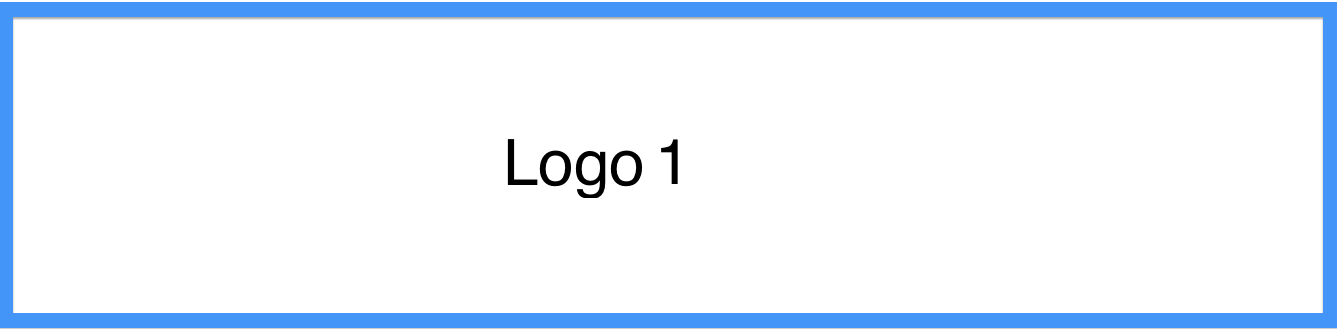
\includegraphics[width=0.4\textwidth,angle=45]{abb/logo1}
 \caption[Beispiel einer Bildbeschreibung]{Beispiel einer Bildbeschreibung\footnotemark}
\label{fig:beispiel1}
\end{figure}
\footnotetext{Bildquelle: Beispiel einer Bildquelle}

% Beispiel für Bildintegration
\begin{figure}[htb]
 \centering
 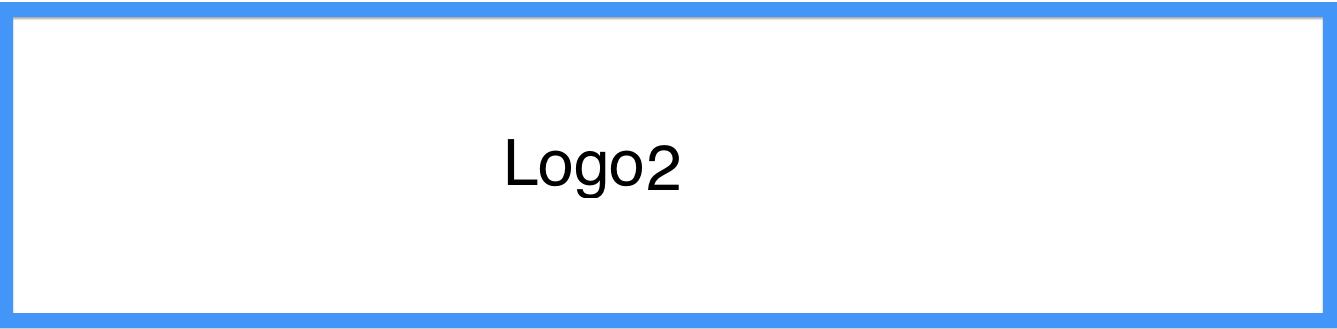
\includegraphics[width=0.3\textwidth,angle=0]{abb/logo2}
 \caption[Beschreibung]{Beschreibung}
\label{fig:Beschreibung}
\end{figure}

% Beispiel: Referenz auf Abbildung
Abbildung~\ref{fig:Beschreibung} [S.\pageref{fig:Beschreibung}]

% Beispiel: Tabelle 
\begin{center}
  \begin{tabular}{ | l | c | }
    \hline
    Überschrift 1 & Überschrift 2 \\ \hline \hline
    Info 1 & Info 2 \\ \hline
    Info 3 & Info 4 \\ \hline
    \hline
    \multicolumn{2}{|c|}{Info in einer Zelle} \\
    \hline
  \end{tabular}
\end{center}


% Beispiel für Quellcode Listings
\lstset{language=xml}
\begin{lstlisting}[frame=htrbl, caption={Die Datei {\normalfont \ttfamily  data-config.xml} dient als Beispiel für XML Quellcode}, label={lst:dataconfigxml}]
<dataConfig>
  <dataSource type="JdbcDataSource" 
              driver="com.mysql.jdbc.Driver"
              url="jdbc:mysql://localhost/bms_db"
              user="root" 
              password=""/>
  <document>
    <entity name="id"
        query="select id, htmlBody, sentDate, sentFrom, subject, textBody
        from mail">
    <field column="id" name="id"/>
    <field column="htmlBody" name="text"/>
    <field column="sentDate" name="sentDate"/>
    <field column="sentFrom" name="sentFrom"/>
    <field column="subject"  name="subject"/>
    <field column="textBody" name="text"/>
    </entity>
  </document>
</dataConfig>
\end{lstlisting}

\lstset{language=java}
\begin{lstlisting}[frame=htrbl, caption={Das Listing zeigt Java Quellcode}, label={lst:result2}]
/* generate TagCloud */
Cloud cloud = new Cloud();
cloud.setMaxWeight(_maxSizeOfText);
cloud.setMinWeight(_minSizeOfText);
cloud.setTagCase(Case.LOWER);
	    
/* evaluate context and find additional stopwords */
String query = getContextQuery(_context);
List<String> contextStoplist = new ArrayList<String>();
contextStoplist = getStopwordsFromDB(query);
	    
/* append context stoplist */
while(contextStoplist != null && !contextStoplist.isEmpty())
  _stoplist.add(contextStoplist.remove(0));
	    
/* add cloud filters */
if (_stoplist != null) {
  DictionaryFilter df = new DictionaryFilter(_stoplist);
  cloud.addInputFilter(df);
}
/* remove empty tags */
NonNullFilter<Tag> nnf = new NonNullFilter<Tag>();
cloud.addInputFilter(nnf);

/* set minimum tag length */
MinLengthFilter mlf = new MinLengthFilter(_minTagLength);
cloud.addInputFilter(mlf);

/* add taglist to tagcloud */
cloud.addText(_taglist);

/* set number of shown tags */	    
cloud.setMaxTagsToDisplay(_tagsToDisplay);
\end{lstlisting}


% Beispiel für Formeln
Die Zuordnung aller möglichen Werte, welche eine Zufallsvariable annehmen kann nennt man \emph{Verteilungsfunktion} von $X$.

\begin{quotation}
Die Funktion F: $\mathbb{R} \rightarrow$ [0,1] mit $F(t) = P (X \le t)$ heißt Verteilungsfunktion von $X$.\footnote{Mustermann, vgl.~\cite{mm2009}~[S.55]}
\end{quotation}

\begin{quotation}
Für eine stetige Zufallsvariable $X: \Omega \rightarrow \mathbb{R}$ heißt eine integrierbare, nichtnegative reelle Funktion $w: \mathbb{R} \rightarrow \mathbb{R}$ mit $F(x) = P(X \le x) = \int_{-\infty}^{x} w(t)dt$ die \emph{Dichte} oder \emph{Wahrscheinlichkeitsdichte} der Zufallsvariablen $X$.\footnote{Mustermann, vgl.~\cite{mf2005}~[S.56]}
\end{quotation}


% einfacher Zeilenabstand
\singlespacing
% Literaturliste soll im Inhaltsverzeichnis auftauchen
\newpage
\phantomsection
\addcontentsline{toc}{section}{Literaturverzeichnis}
% Literaturverzeichnis anzeigen
\renewcommand\refname{Literaturverzeichnis}
\bibliography{Hauptdatei}

%% Index soll Stichwortverzeichnis heissen
% \newpage
% % Stichwortverzeichnis soll im Inhaltsverzeichnis auftauchen
% \addcontentsline{toc}{section}{Stichwortverzeichnis}
% \renewcommand{\indexname}{Stichwortverzeichnis}
% % Stichwortverzeichnis endgültig anzeigen
% \printindex

\onehalfspacing
% evtl. Anhang
\newpage
\phantomsection
\addcontentsline{toc}{section}{Anhang}
\fancyhead[L]{Anhang} %Kopfzeile links
\subsection*{Anhang}
\label{anhang}
%TODO: Anhang Fixen
\appendix
\section{Organigramm}
\label{abb:Organigramm}
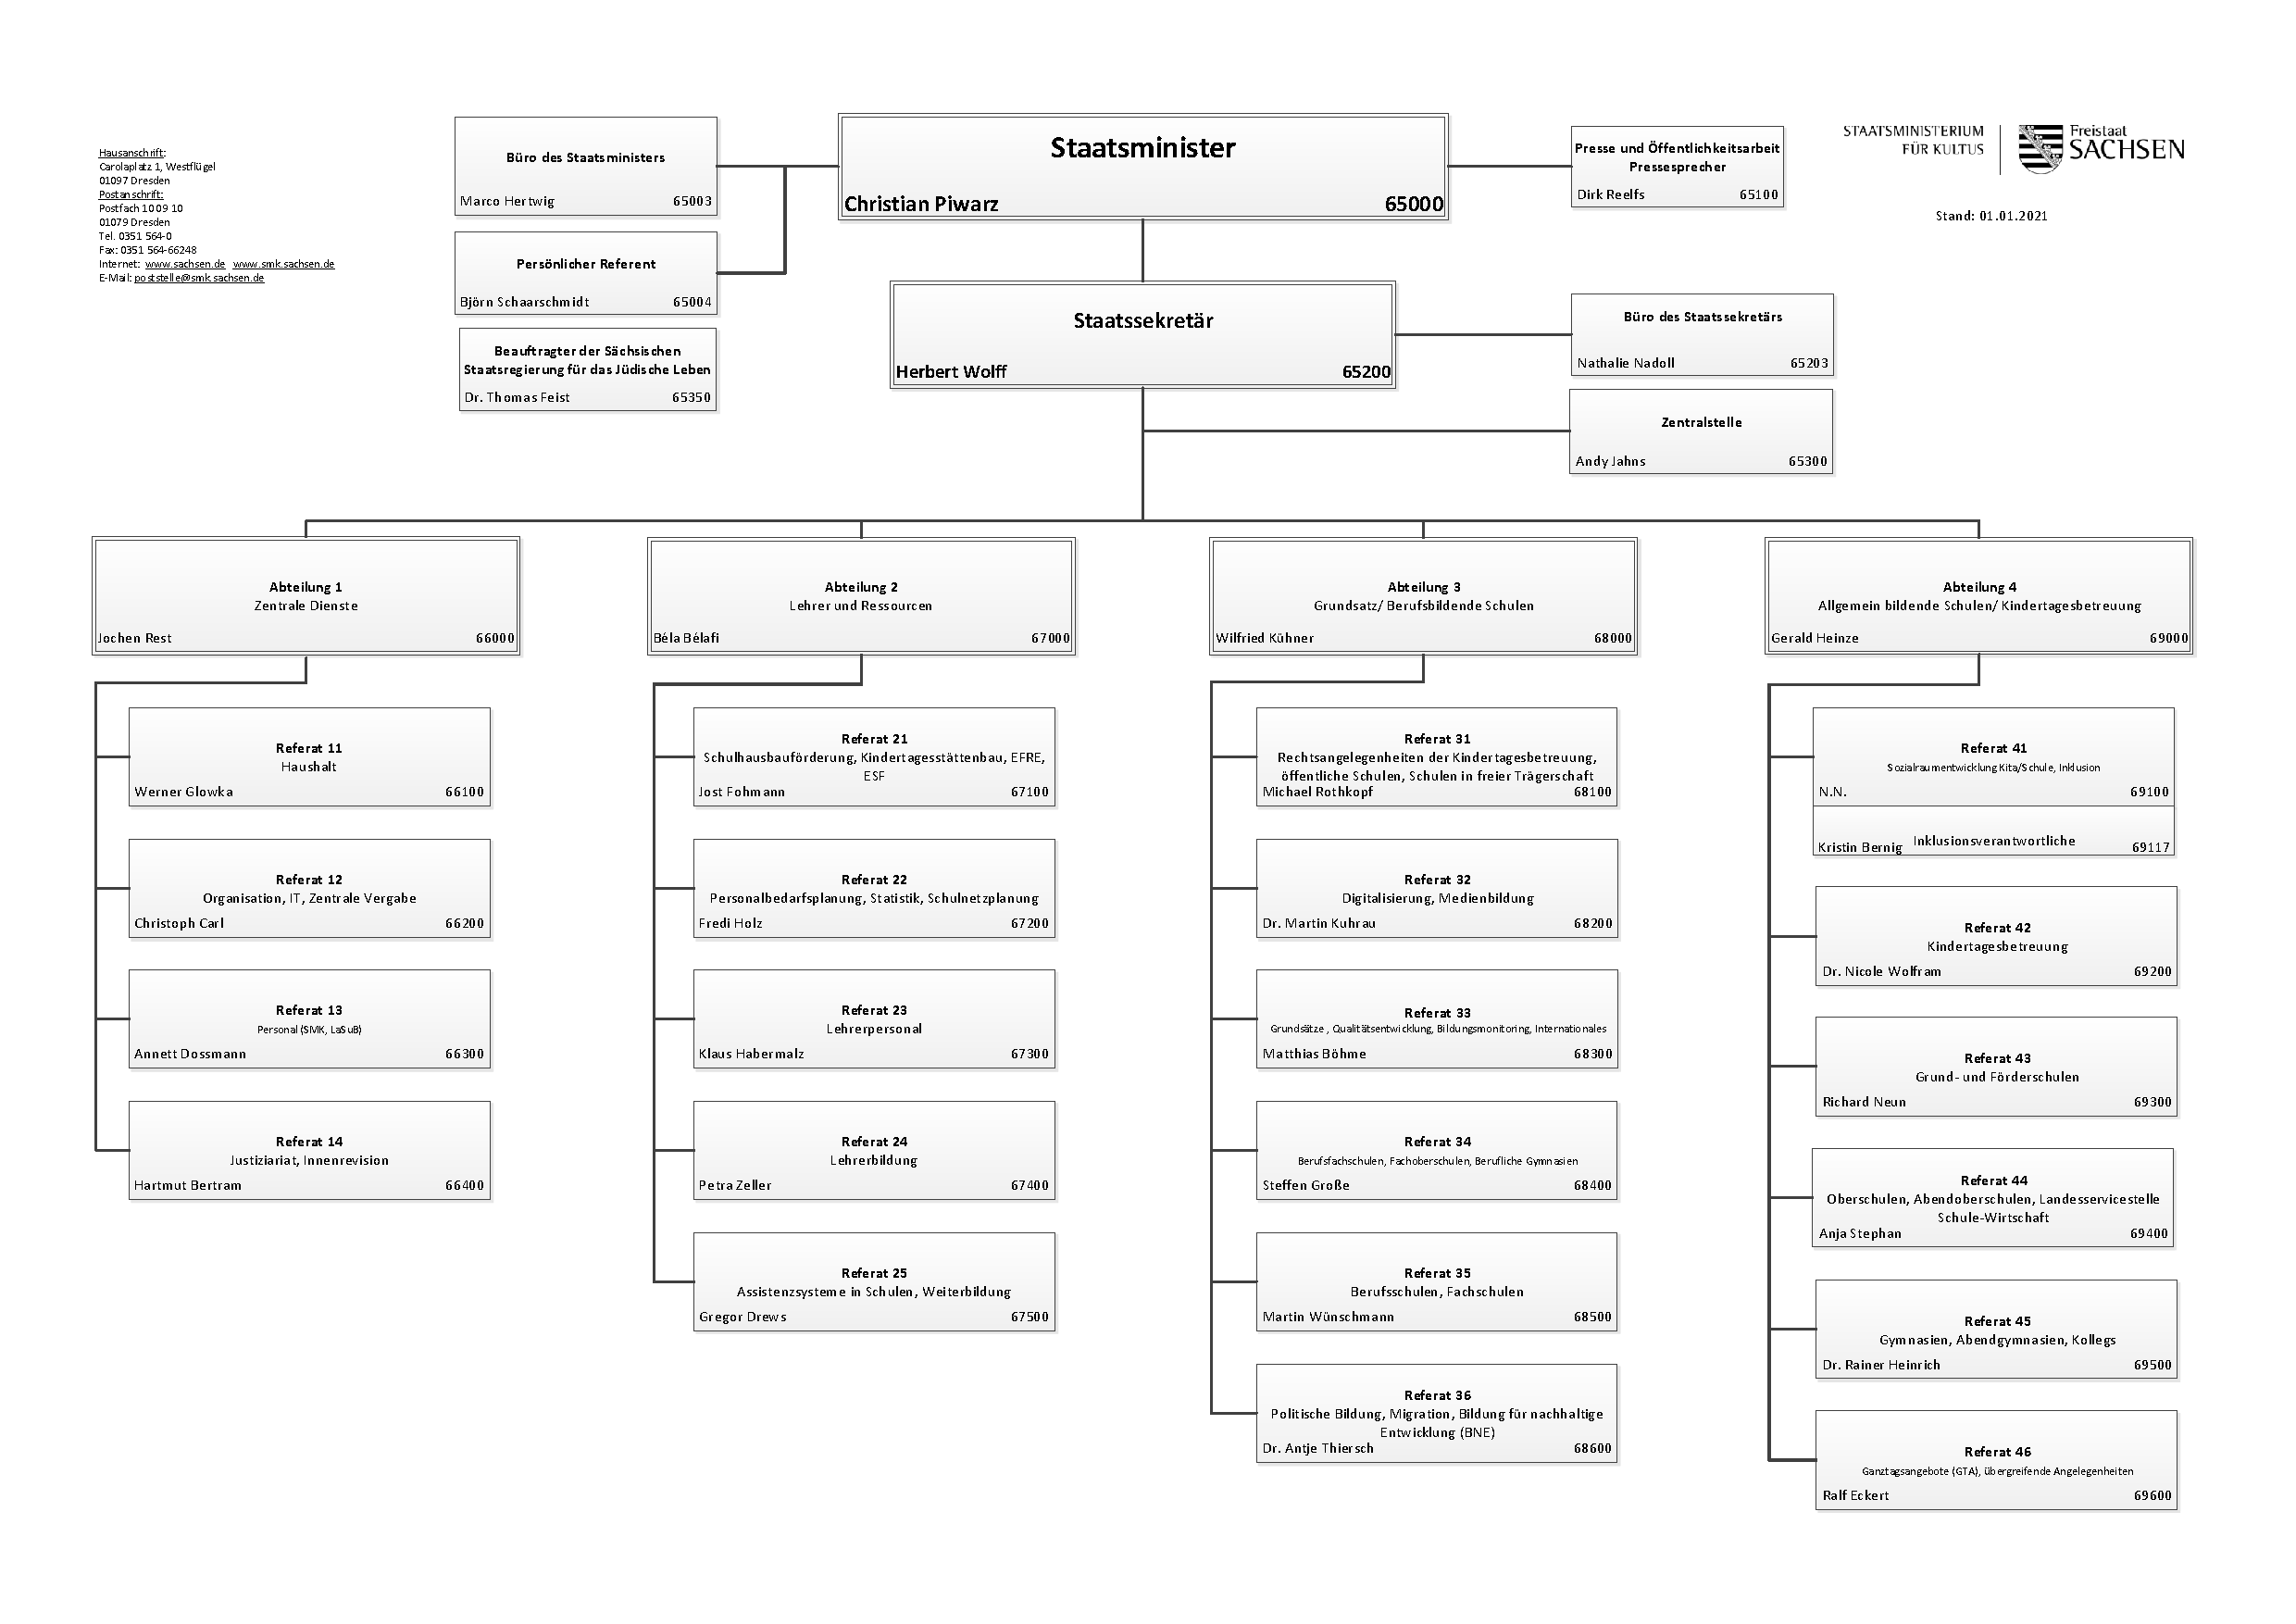
\includegraphics[angle=90, page=1,height=0.90\textheight, keepaspectratio]{anhang/abb/21_01_06_Organigramm_SMK.pdf}

\section{Gantt}
\label{abb:Gantt}
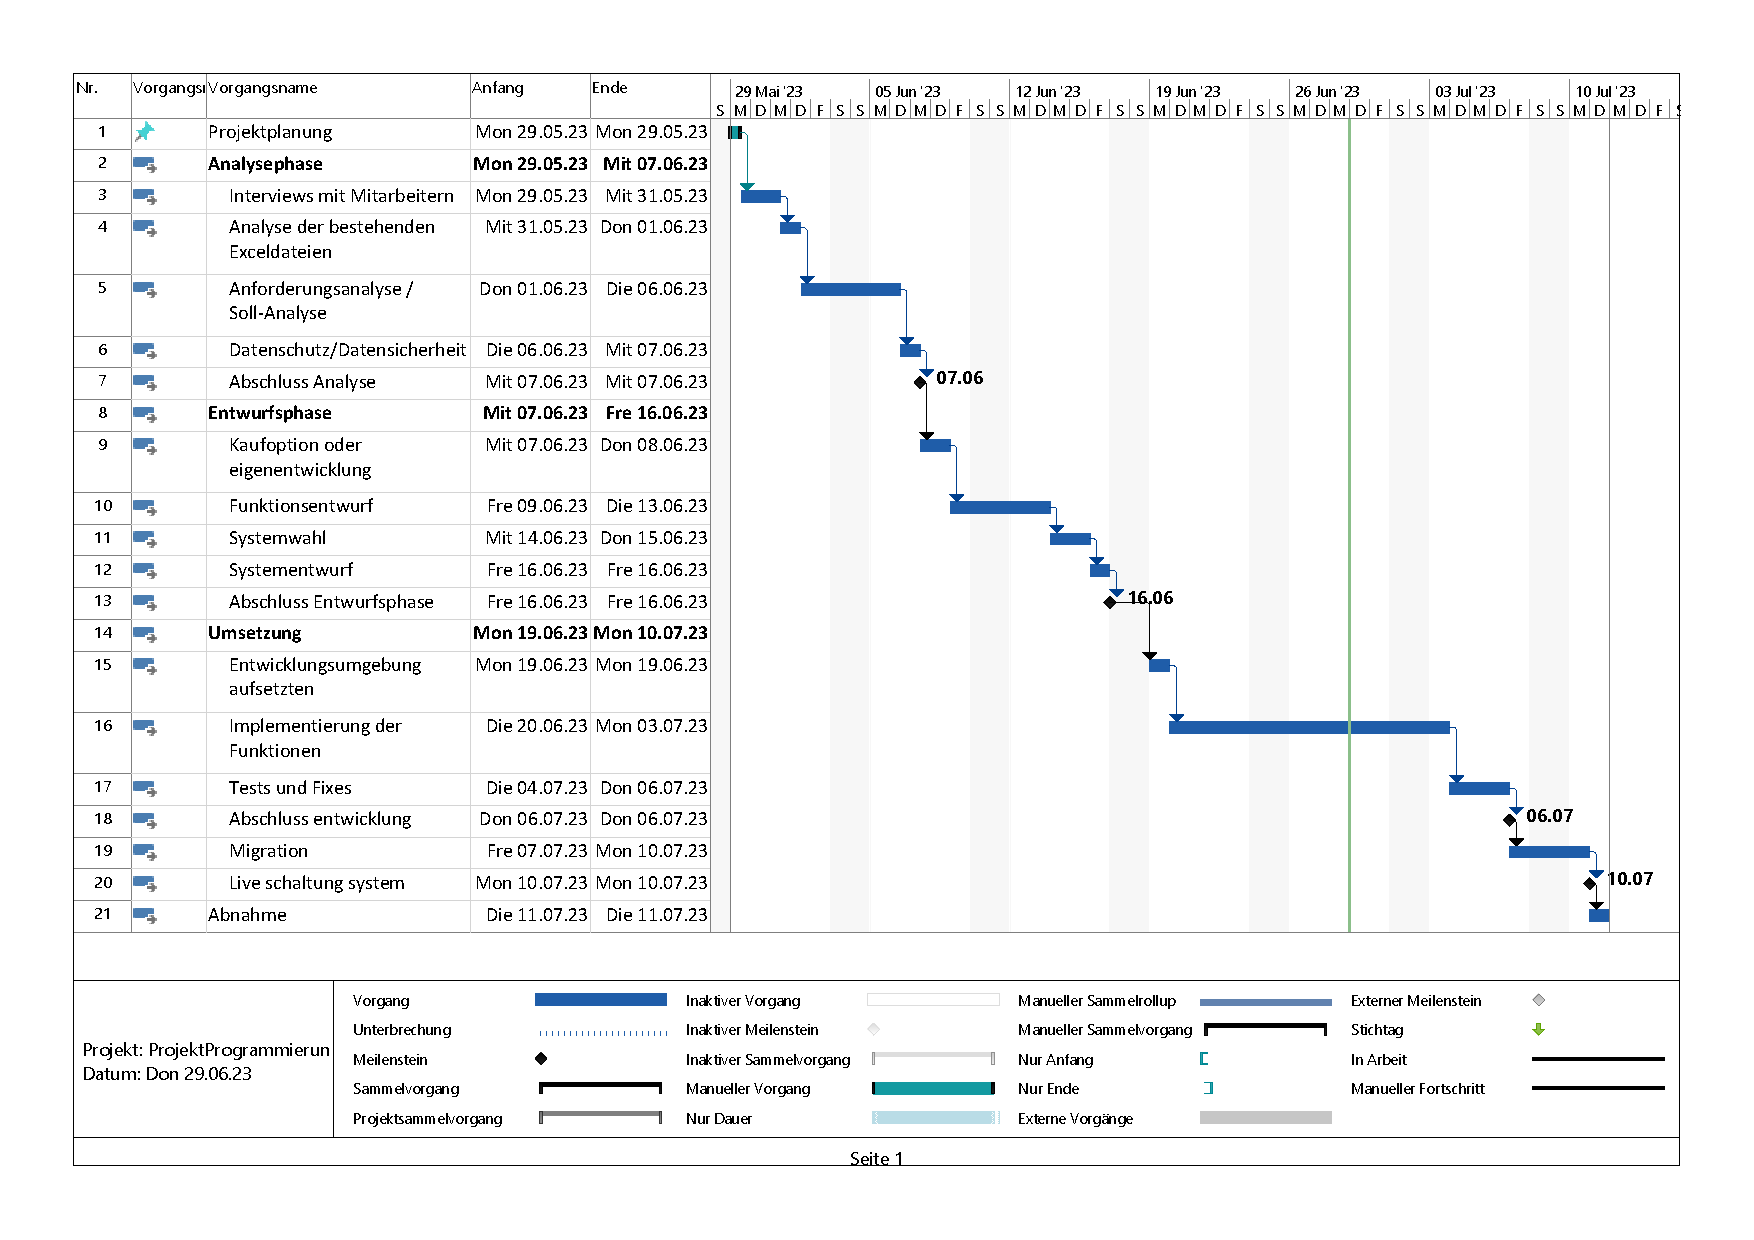
\includegraphics[angle=90, page=1,height=0.90\textheight, keepaspectratio]{anhang/abb/ProjektProgrammierungZeitplan.pdf}

\section{Ausgangstabelle}
\label{abb:Ausgangstabelle}
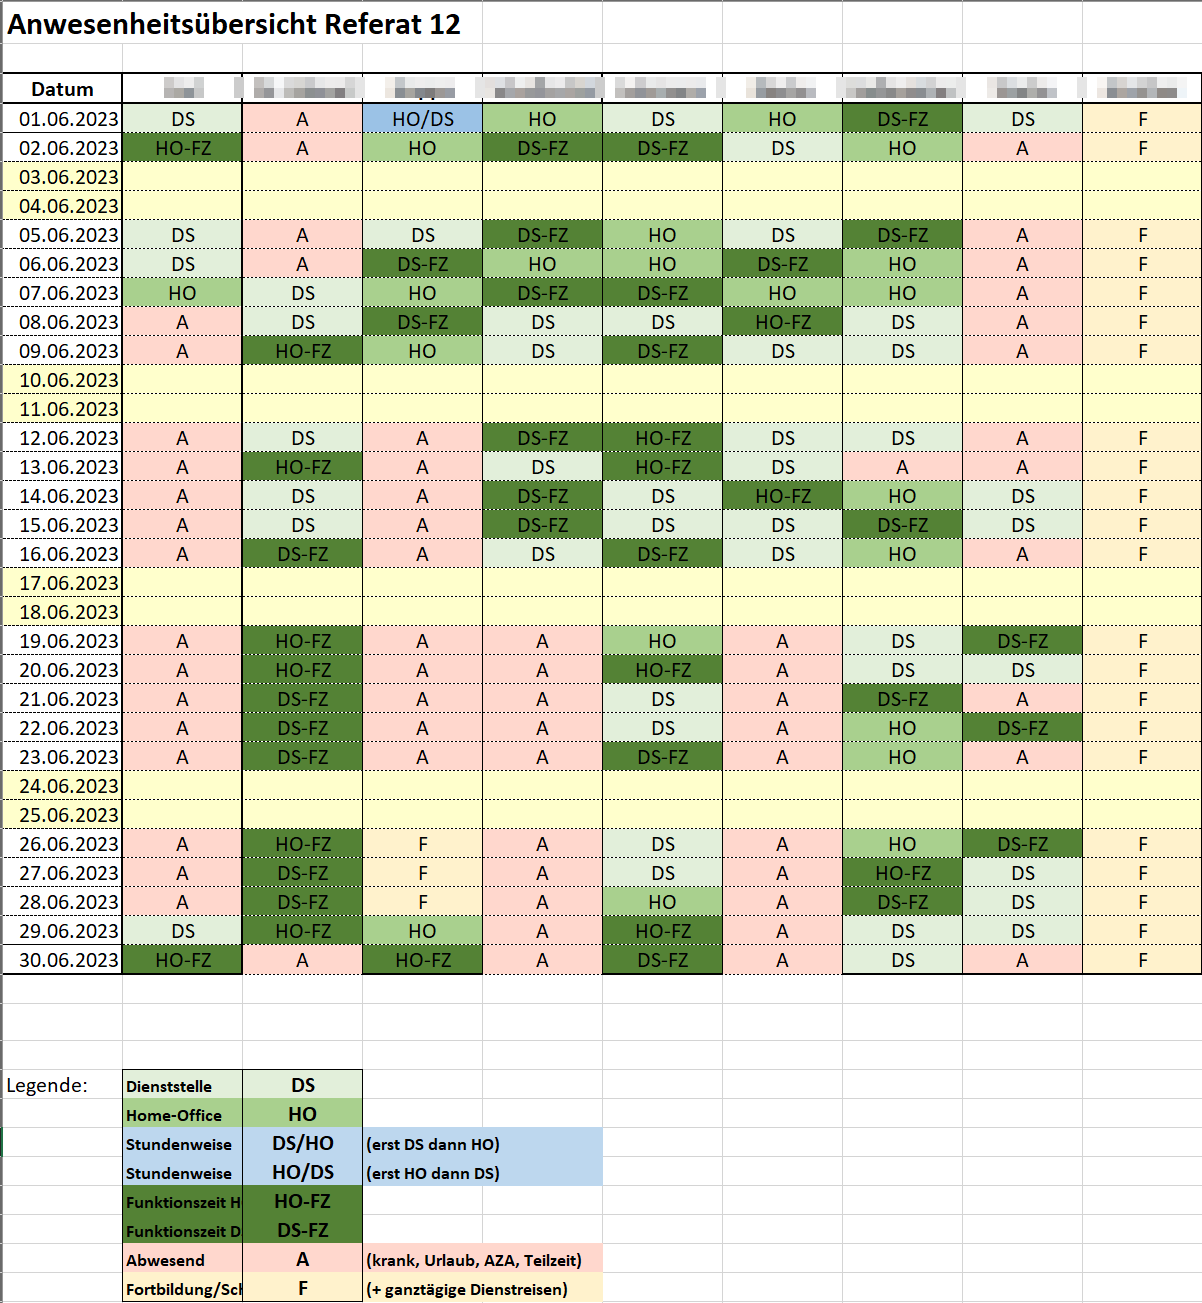
\includegraphics[page=1,height=1\textwidth]{anhang/abb/Tabelle.png}


\begin{figure}[htb]
    \centering
    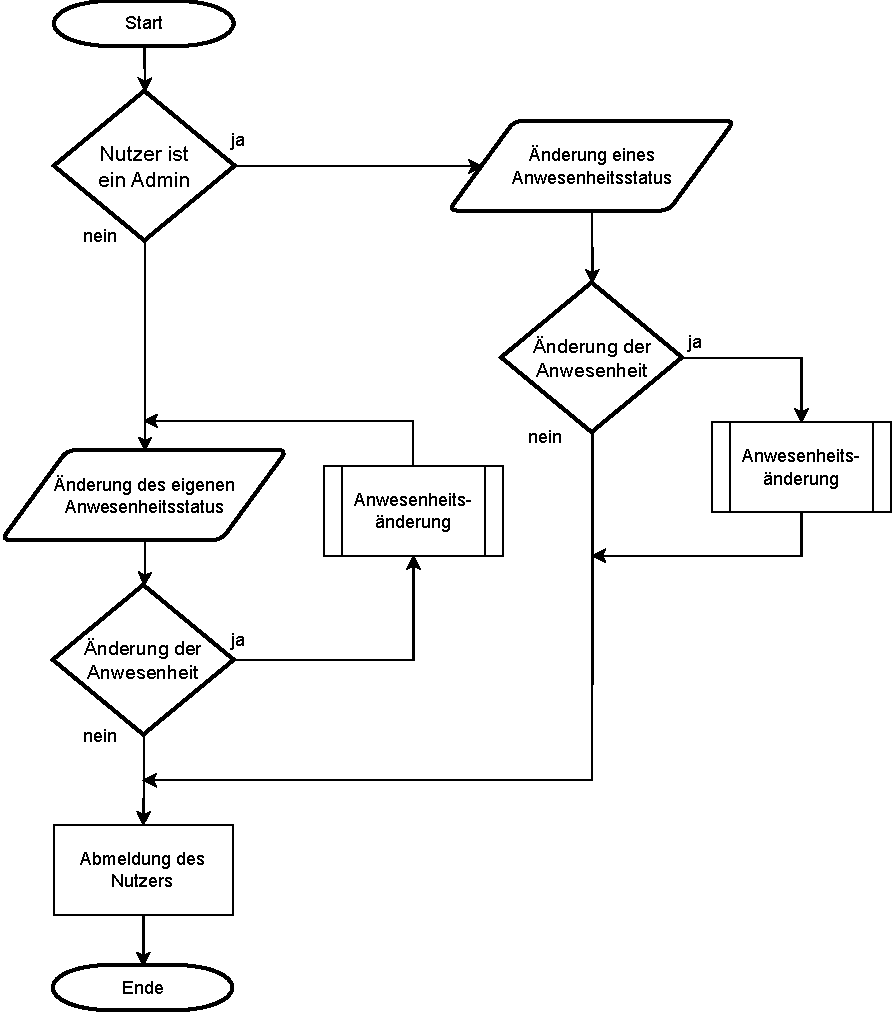
\includegraphics[width=0.9\textwidth,angle=0]{anhang/abb/PAP_Kurz.pdf}
    \caption[Beschreibung]{PAP änderungsvorgang von Anwesenheiten}
    \label{abb:PAP}
\end{figure}

\begin{figure}[htb]
    \centering
    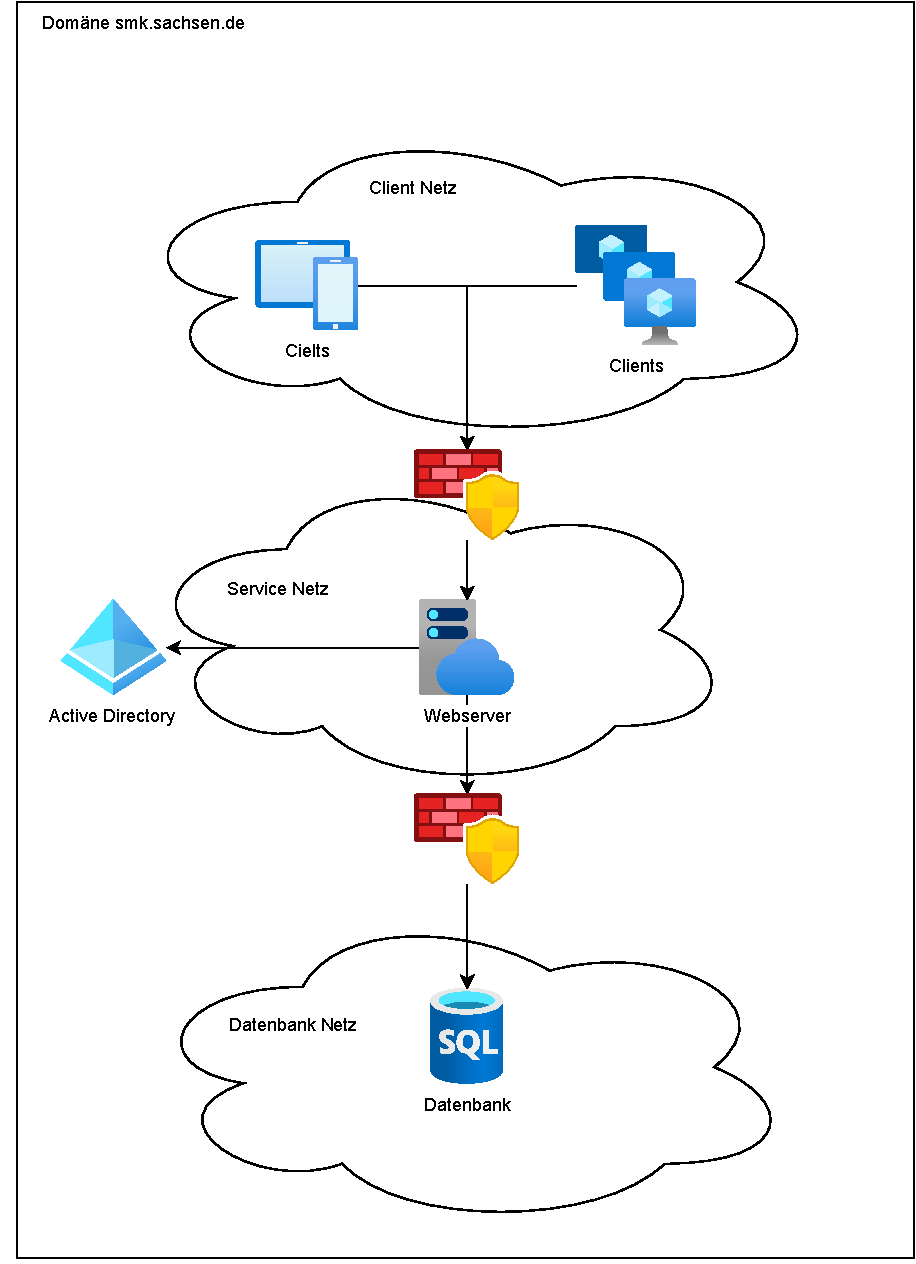
\includegraphics[width=0.9\textwidth,angle=0]{anhang/abb/Systemarchitektur.pdf}
    \caption[Beschreibung]{Systemarchitektur}
    \label{abb:Systemarchitektur}
\end{figure}

% Eidesstattliche Erklärung
\newpage
\phantomsection
\addcontentsline{toc}{section}{Eidesstattliche Erklärung}
\section*{Selbstständigkeitserklärung }
\thispagestyle{empty}

\begin{verbatim}

\end{verbatim}

\begin{LARGE}Erklärung zur selbstständigen Anfertigung der Arbeit \end{LARGE}
\begin{verbatim}


\end{verbatim}
Ich versichere, dass ich die Arbeit selbstständig angefertigt und keine anderen als die angegebenen Hilfsmittel benutzt habe. Wörtlich oder sinngemäß aus anderen Quellen übernommene Textstellen, Bilder, Tabellen u. a. sind unter Angabe der Herkunft kenntlich gemacht. Weiterhin versichere ich, dass diese Arbeit oder eine ähnliche Arbeit mit in Teilen wesentlicher Inhaltsübereinstimmung noch keiner anderen Prüfungsbehörde vorgelegt wurde.





\begin{flushleft}Dresden, am 19.07.2023:\end{flushleft} 
\begin{flushright}Martin Lee Starke\end{flushright}




% leere Abschlussseite
\newpage
\thispagestyle{empty} % erzeugt Seite ohne Kopf- / Fusszeile
\mbox{}

\end{document}
